\documentclass{article}
\usepackage{amsmath}
\usepackage{amsfonts}
\usepackage[a4paper,width=140mm,top=15mm,bottom=15mm]{geometry}
\usepackage{hyperref}
\usepackage{mathtools}
\usepackage{graphicx}
\graphicspath{ {./figures/} }

\hypersetup{
    colorlinks,
    citecolor=black,
    filecolor=black,
    linkcolor=black,
    urlcolor=black
}

\DeclareUnicodeCharacter{2212}{-}




\title{Esercizi}
\author{Michele Leigheb}
\date{}
\begin{document}
\maketitle
\tableofcontents{}
\section{Complessi}
\begin{itemize}
	\item \(\displaystyle 2^{(a+ib)} = 2^a (\cos(b \ln(2)) + i\sin(b \ln(2))) \)
	\item \(\displaystyle 3^{(a+ib)} = 3^a (\cos(b \ln(3)) + i\sin(b \ln(3))) \)
	\item \(\displaystyle e^{(a+ib)} = e^a (\cos(b)) + i\sin(b) \)
	\item \(\displaystyle \alpha^{(a+ib)} = e^{\alpha} (\cos(b)\ln(\alpha)) + i\sin(b\ln(\alpha)) \)
\end{itemize}



\section{Esercizi}

\subsection{$ s^{2} + 1 $}
Il grafico di bode è:
\[ W(s) = \frac{s^{2} + 1}{s^{2} \left(s + 1\right)^{2}} \]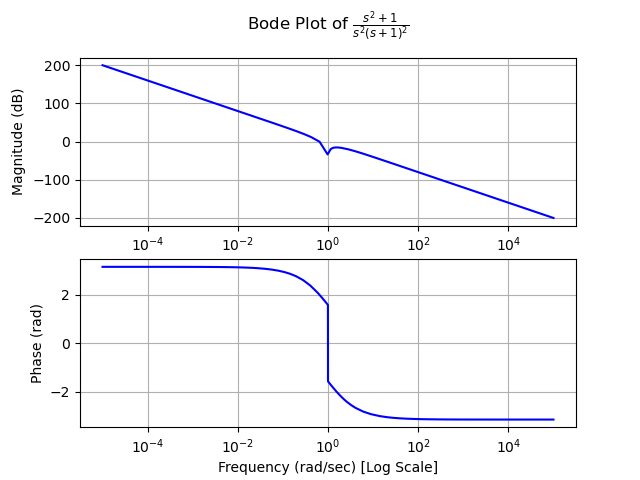
\includegraphics[scale = 0.5]{figures/bode_2948953.png}


Il grafico di Nyquist è:
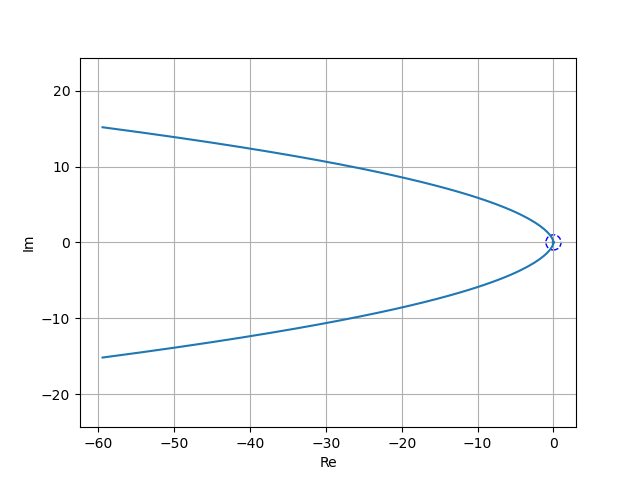
\includegraphics[scale = 0.5]{figures/nyquist_1238369.png}nel tempo continuo è \[ \left(2 t + \left(t - 2\right) e^{t} + 2\right) e^{- t} \theta\left(t\right) \]



























\end{document}
